\section{会员}

\subsection{登录}
\begin{figure}[H]
	\centering
	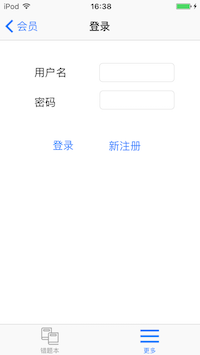
\includegraphics{img/27.png}
	\caption{登录}
	\label{img27}
\end{figure}
在购买会员前,可以先注册登录。点击会员页面右上角,进入登录页面,如图(\ref{img27}),输入用户名和密码登录。如果还没有用户名和密码,点击“新注册”。

本公司产品通用一套用户名和密码。如果注册过,直接用以前的用户名和密码登录即可。

\subsection{注册}
\begin{figure}[H]
	\centering
	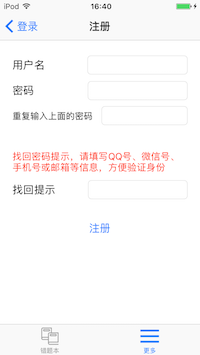
\includegraphics{img/28.png}
	\caption{注册}
	\label{img28}
\end{figure}
如图(\ref{img28}),输入用户名、密码、找回密码提示等信息,点击“注册”。

注意:2次密码输入要一致。找回密码提示需要填写QQ号、微信号、手机号码、邮箱,客服依据填写信息确定用户是否是本人后,提供服务。

本公司产品通用一套用户名和密码。如果提示用户名已经被使用,请确认是否在本公司其他产品中注册过。如果注册过,直接用以前的用户名和密码登录即可。

\subsection{升级会员}
\begin{figure}[H]
	\centering
	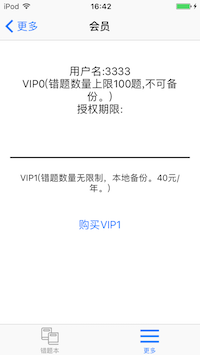
\includegraphics{img/29.png}
	\caption{升级会员}
	\label{img29}
\end{figure}
如图(\ref{img29}),可以直接升级会员。付费后,退出当前页面,重新进入。

\begin{itemize}
	\item VIP0,默认,错题数量上限100题,不可本地备份。
	\item VIP1,错题数量无限制,可本地备份。可注册登录后购买,40元/年,限本人使用。
\end{itemize}

\subsection{绑定用户}
如果先购买了会员,会分配一个随机用户名。可以后续修改绑定成自己的用户名,操作类似注册。推荐绑定成自己的用户名。

%\section{分享}
%\begin{figure}[H]
%	\centering
%	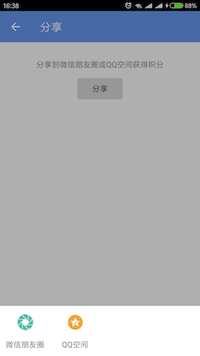
\includegraphics{img/30.png}
%	\caption{分享}
%	\label{img30}
%\end{figure}
%如图(\ref{img30}),可分享到微信朋友圈、QQ空间。每次成功分享后,分享积分+1
%\begin{itemize}
%	\item 分享积分累计7分后,可以免费备份1次。备份后,累计分-7分。
%	\item 当日分享后,可以无限制添加错题。
%\end{itemize}

\section{备份}
\begin{figure}[H]
	\centering
	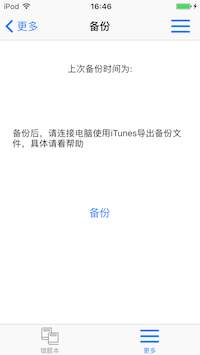
\includegraphics{img/31.png}
	\caption{备份}
	\label{img31}
\end{figure}
如图(\ref{img31}),积累的错题,是珍贵的学习资料,不容有失。

%VIP1会员或分享积分7分以上,可以进行备份。
VIP1会员,可以进行备份。

重要:备份后,请使用电脑上的iTunes导出备份文件wgctb\_xxx.bak,否则数据会随着app卸载,也被删除。具体操作可查看苹果官方帮助[关于 iPhone、iPad 和 iPod touch 上的“文件共享”],链接地址为:\url{https://support.apple.com/zh-cn/HT201301}

右上角菜单
\begin{itemize}
	\item 整理数据(删除错题、错题本后,备份文件大小不见减少时,可以使用整理数据功能,压缩备份文件大小)。请先备份导出一次,然后整理数据。可能需要大量时间,请耐心等待。
	\item 清理备份(删除所有bak备份文件,建议在备份文件已经导出后操作)
\end{itemize}

\section{恢复备份}
\label{restore}
\begin{figure}[H]
	\centering
	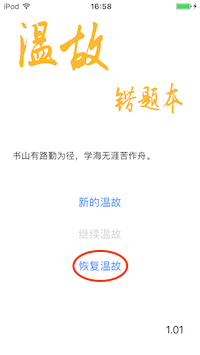
\includegraphics{img/2.png}
	\caption{进入恢复}
	\label{img2}
\end{figure}

重新安装app后,可以选择“恢复温故”,如图(\ref{img2}),进入恢复备份页面,如图(\ref{img3})

\begin{figure}[H]
	\centering
	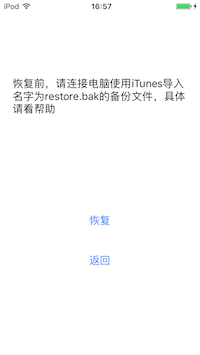
\includegraphics{img/3.png}
	\caption{恢复}
	\label{img3}
\end{figure}

选择一个历史备份,重命名为restore.bak,使用电脑上的iTunes导入,具体操作可查看苹果官方帮助[关于 iPhone、iPad 和 iPod touch 上的“文件共享”],链接地址为:\url{https://support.apple.com/zh-cn/HT201301},点击“恢复”,让错题本数据恢复到备份时的状态。
\section{升级}
可以先备份导出一次。升级app,请在appstore中,直接安装新的app版本。千万不要先删除,后安装,这样会丢失所有错题数据。